%% This is an example file to show how to use JASA_manu.sty and related 
%% files written by Eric C. Anderson.  It's sort of a fly-by-night endeavor,
%% but I got it to work for me!!


\documentclass[12pt, letter]{article}\usepackage[]{graphicx}\usepackage[]{color}
%% maxwidth is the original width if it is less than linewidth
%% otherwise use linewidth (to make sure the graphics do not exceed the margin)
\makeatletter
\def\maxwidth{ %
  \ifdim\Gin@nat@width>\linewidth
    \linewidth
  \else
    \Gin@nat@width
  \fi
}
\makeatother

\definecolor{fgcolor}{rgb}{0.345, 0.345, 0.345}
\newcommand{\hlnum}[1]{\textcolor[rgb]{0.686,0.059,0.569}{#1}}%
\newcommand{\hlstr}[1]{\textcolor[rgb]{0.192,0.494,0.8}{#1}}%
\newcommand{\hlcom}[1]{\textcolor[rgb]{0.678,0.584,0.686}{\textit{#1}}}%
\newcommand{\hlopt}[1]{\textcolor[rgb]{0,0,0}{#1}}%
\newcommand{\hlstd}[1]{\textcolor[rgb]{0.345,0.345,0.345}{#1}}%
\newcommand{\hlkwa}[1]{\textcolor[rgb]{0.161,0.373,0.58}{\textbf{#1}}}%
\newcommand{\hlkwb}[1]{\textcolor[rgb]{0.69,0.353,0.396}{#1}}%
\newcommand{\hlkwc}[1]{\textcolor[rgb]{0.333,0.667,0.333}{#1}}%
\newcommand{\hlkwd}[1]{\textcolor[rgb]{0.737,0.353,0.396}{\textbf{#1}}}%

\usepackage{framed}
\makeatletter
\newenvironment{kframe}{%
 \def\at@end@of@kframe{}%
 \ifinner\ifhmode%
  \def\at@end@of@kframe{\end{minipage}}%
  \begin{minipage}{\columnwidth}%
 \fi\fi%
 \def\FrameCommand##1{\hskip\@totalleftmargin \hskip-\fboxsep
 \colorbox{shadecolor}{##1}\hskip-\fboxsep
     % There is no \\@totalrightmargin, so:
     \hskip-\linewidth \hskip-\@totalleftmargin \hskip\columnwidth}%
 \MakeFramed {\advance\hsize-\width
   \@totalleftmargin\z@ \linewidth\hsize
   \@setminipage}}%
 {\par\unskip\endMakeFramed%
 \at@end@of@kframe}
\makeatother

\definecolor{shadecolor}{rgb}{.97, .97, .97}
\definecolor{messagecolor}{rgb}{0, 0, 0}
\definecolor{warningcolor}{rgb}{1, 0, 1}
\definecolor{errorcolor}{rgb}{1, 0, 0}
\newenvironment{knitrout}{}{} % an empty environment to be redefined in TeX

\usepackage{alltt}
\usepackage[top=1in, bottom=1in, left=1in, right=1in]{geometry}
\usepackage{graphicx}
\usepackage{float}
\usepackage{amsmath, amssymb, mathtools }
\usepackage{enumerate}
\usepackage{array}
\usepackage{fancyhdr}
\usepackage[hypcap]{caption}
\usepackage{verbatim}
\usepackage{color}
\usepackage{pstricks}
\usepackage{psfrag}
\usepackage{epsfig,epsf}
\usepackage{setspace}
\doublespacing
%% THE NEXT TWO LINES INSERT THE PACKAGES FOR JASA FORMAT:
\usepackage[default]{jasa_harvard}    % 	for formatting citations in text
\usepackage{JABES_manu}


%% CHANGING THE 'AND' IN THE HARVARD BIBLIOGRAPHY PACKAGE TO WHAT IT OUGHT TO BE
\renewcommand{\harvardand}{and}


%% Here is a hand-formatted bibliography reference list entry.
%% The command should be included in the NOTE field of the entry in the .bib file
\IfFileExists{upquote.sty}{\usepackage{upquote}}{}
\begin{document}


\title{ Backward Selection Procedures to  Detect Differential Expressed Genes in RNA-Seq Data
Accounting for Nuisance Covariates}
\author{Yet Nguyen and Dan Nettleton\\
Department of Statistics, 
Iowa State University, Ames, IA 50010\\ 
email: \texttt{ntyet@iastate.edu}
}

\maketitle


%% ABSTRACT

%
\begin{center}
\textbf{Abstract}
\end{center}
Differential Expression Analysis of RNA-Seq data can often be complicated by the presence of nuisance factors that arise due to experimental design limitations and heterogeneity of experimental units that can be seen in continuous and categorical covariates measured for each experimental unit and/or RNA sample. The analysis is typically done by including or ignoring all nuisance covariates. Some drawbacks of those approaches are that the False Discovery Rate (FDR) is usually too conservative or too liberal, and the power of detecting differentiallly expressed genes is very small. To address these shortcomings, we develop two backward selection procedures to pick up the most significant covariates, which in turn are combined in a optimal model  to identify differentially expressed genes. The proposed methods are then applied to RNA-Seq data from Residual Feed Intake project. Furthermore, simulation results from real data show that our proposed methods outperform the traditional strategies commonly used to detect differentially expressed genes accounting for nuisance covariates, which are methods that include or exclude all covariates.

\vspace*{.3in}

\noindent\textsc{Keywords}: {Backward Model Selection, Grenander Estimator,  False Discovery Rate, Partial AUC, Kolmogorov-Smirnov Statistics, RNA-Seq, Nuisance Covariates, Differential Expression Analysis.}

%

\section{ Introduction}
A nuisance variable, or confounded variable, is an undesirable variable that is associated with the outcome within an experimental study and is typically of no interest to the researcher. It might be a feature of the experimental unit under study or any unintended influence on an experimental manipulation. A nuisance variable causes greater variability in the distribution of a sample's outcome and affects all the groups measured within a given sample. In the situation of RNA-Seq experiment, accounting for nuisance variables is becoming increasingly important due to the expensive cost of this high throughput sequencing technology.

As a specific motivation example, consider the RNA-Seq experiment conducted by Iowa State University  researchers to examine gene expression in two Yorkshire residual feed intake (RFI) pig \emph{lines} feeded either by \emph{high fiber-low energy diet} or \emph{low fiber-high energy diet}. Illumina RNA-Seq was used to measure gene expression of total 31 pigs  of full 2-factor factorial design $\emph{Line} \times \emph{Diet}$ (one sample form a pig is excluded due to its low RNA quality). 

The main purpose of the experiment  can be described as follows. Prior of the experiment, it was known that feed is the largest cost of US pork producer, representing about 60 \% of the total cost. Hence, knowledge on efficiency of nutrient utilization and development of new technologies and mechanisms for improving feed efficiency (FE) is essential to the long term competitiveness of the US pork industry and for improving the sustainability of food supplies. In contrast to the mechanisms that govern  growth and development, our perception of the biological mechanisms regulating FE is limited. Therefore there is a critical need to define the mechanisms that regulate FE. \citeasnoun**{kochetal1963}  suggested the concept of RFI to measure FE in cattle. RFI is the difference between observed feed intake and expected feed intake based on average daily gain and back fat. Efficient animals have a low negative RFI, i.e., they consume less feed than expected for their rate of gain, and reversely, animals with high positive RFI consume more feed than expected. RFI is the unique measure of FE because it is regarded as true difference in the ability of animals to use feed energy for the metabolic processes of maintenance and growth. However, measuring RFI is expensive and time-consuming. The purpose of the study is to use whole blood from 4-5 week-old pigs  to identify differentially expressed genes between two Yorkshire lines of pigs divergently based on RFI, with the long term goal that is to  develop useful biomarkers for FE. 

Blood samples were collected into Tempus tubes for long-term storage and EDTA tubes for complete blood count (CBC) test from 233 piglets  (Generation 9, at 35-42 days of age) of the two Yorkshire lines of pigs divergently selected for FE 
based on RFI, the low RFI line and the high RFI line. The CBC of all blood samples eventually is measured. These animals were later randomly assigned to two \emph{diets} of different fiber and energy content, and each pig’s RFI was measured on FIRE feeders. Blood samples of 8 animals of extremely low RFI in the low RFI line and extremely high RFI in the high RFI line on each diet were selected for RNA-sequencing, with one sample later dropped due to low RNA quality. RNA samples were prepared and globin transcripts were depleted by an RNase H-mediated method before RNA 
sequencing. One hundred bp paired-end sequencing was run on the Illumina HiSeq 2000 platform. Reads were mapped to the pig reference genome (Sscrofa10.2.76) using aligner STAR after quality trimming and featureCounts was used to get read 
counts for each gene. In summary, the main effect of interest is RFI Line effect (Line), and there are 13 nuisance covariates including Diet, RFI value, 
CBC values (lymphocyte, neutrophil, monocyte, basophil and eosinophil), and some technical variables such as processing batch (Block), processing order (Order), RNA concentration before and after globin depletion (Concb, Conca), RNA Integrity Number before and after globin depletion (RINb, RINa). Finally, we obtain RNA-Seq data consisting of 25320 genes and 31 samples. After excluding small expression genes, the RNA-Seq data have 12280 genes and 31 samples. 
Using QuasiSeq \citeasnoun**{lundetal2012}, we conduct preliminary analysis based on the traditional approaches which are the one including all nuisance covariates and the one ignoring all nuisance covariates. The approach including all nuisance covariates can detect 2  differentially expressed genes  between 2 RFI lines when controlling FDR at 5\%.  The approach excluding all nuisance covariates can detect  233 differentially expressed genes when controlling FDR at 5\%. Figure \ref{figure1}  shows histograms of $p$-values for testing the significant of Line effect based on these two approaches. 
\begin{figure}[H]
\centering
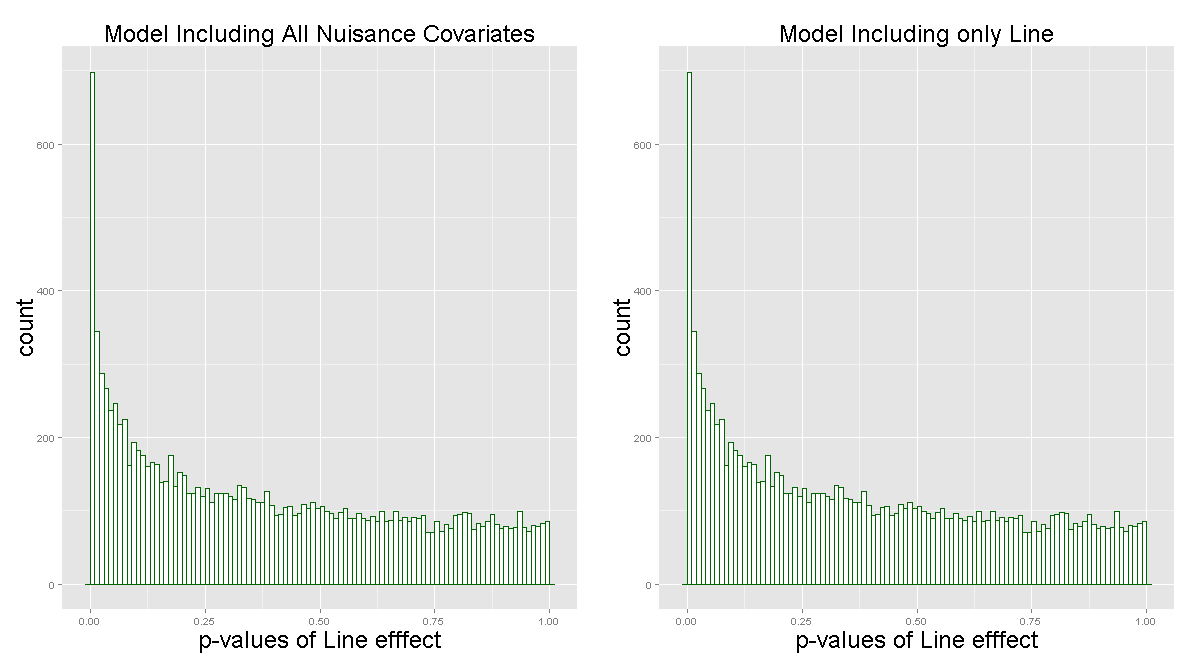
\includegraphics[scale = 0.22]{intro_plot.png}
\caption{The left plot is the histogram of $p$-values of Line effect based on the approach including Line effect and all nuisance covariates. The right plot is the histogram of $p$-values of Line effect based on the approach excluding all nuisance covariates.}
\label{figure1}
\end{figure}

This article focuses on backward model selection procedures to  choose the model which is  optimal for differential expression analysis in the sense that the power of detecting differentially expressed genes is largest while FDR is controlled at a desired level. The basis method is described in Section 2. Section 2.1 contains preliminary of probability model for RNA-Seq count data. Section 2.2 mentions definition of FDR.  Section 2.3 reviews the results on Grenander estimator of non-increasing probability distribution function. Section 2.4 proposes a Kolmogorov-Smirnov  type statistic between two distributions. Section 2.5 contains the description of two backward selection procedures, one using Kolmogorov-Smirnov  type statistic between Grenander estimator and uniform distribution, the other using the number of $p$-values less than 0.05. Section 3 demonstrates these approaches by analyzing RFI RNA-Seq data described above. Section 4 devotes to a simulation study that compares the proposed approaches with the traditional approaches which are including or excluding all nuisance covariates. The article concludes in Section 5. 
\section{ Methods}
\subsection{ Model for Count Data}
Let $y_{gij}$ be the count of gene $g$ from experimental unit $j$ of treatment group $i$ where $i = 1,2$; $j = 1, \dots, n_i$; $g = 1, \dots, m$. As is popular in RNA-Seq data analysis, we assume that the data for gene $g$ ($i = 1, 2$, $j = 1, \dots, n_i$) are independent and have negative binomial distribution $y_{gij} \sim \mbox{NB}(\mu_{gij}, \omega_g)$, where $\mu_{gij}$ is the mean and $\omega_g$ is the dispersion parameter of the negative binomial distribution, i.e., the mean-variance relation is $\mbox{Var}(y_{gij}) = \mu_{gij} + \omega_g \mu_{gij}^2$. Suppose that $x_{0ij}$ is the value of treatment indicator of 
experimental unit $j$ in treatment group $i$, $x_{lij}$ is the value of $l$-th nuisance covariate corresponding to the experimental unit $j$ in treatment group $i$ ($l = 1, \dots, k$), and 
\[
\log(\mu_{gij}) = o_{ij} + \alpha_{g} + \beta_{0g}x_{0ij} + \beta_{1g}x_{1ij} + \cdots + \beta_{kg}x_{kij}, \quad g = 1, \dots, m; i = 1, 2; j = 1, \dots, n_i.
\]

We are interested in testing the treatment effect, i.e., $H_0: \beta_{0g} = 0$ vs. $H_a: \beta_{0g} \neq 0$ for $g =  1, \dots, m$, in the same time accounting for the nuisance covariates under the testing $H_{l0}: \beta_{lg} = 0$ vs $H_{la}: \beta_{jg} \neq 0$. Many methods to detect differential expression genes have been proposed in literature. In the situation involving nuisance covariates, we use QuasiSeq (\citeasnoun**{lundetal2012}) to obtain the $p$-values of the treatment main effect tests and nuisance covariates tests. For more details of QuasiSeq method in comparison with other popular RNA-Seq analysis methods,  we refer interested readers to the paper by \citeasnoun**{lundetal2012} and references therein.

\subsection{ False Discovery Rate}
False discovery rate (FDR) is a popular error rate criterion  in multiple hypothesis testing.  It is first introduced in the well-known paper by \citeasnoun**{BH1995}. This approach was shown to have better power comparing to the traditional familywise error rate control like Bonferroni correction. The FDR is defined as the expected False Discovery Proportion (FDP) which is the  proportion of falsely rejected hypotheses. In particular, consider the problem of testing $m$ null hypotheses, of which $m_0$ are true. We assume that the $m$ hypothesis tests have corresponding $p$-values $p_1, \dots, p_m$. Table \ref{tab:t1} summarizes the outcome of hypotheses in a traditional form. 

\begin{table}
\centering
\begin{tabular}{|c|cc|c|}
\hline
& Declared non-significant   & Declared significant & Total \\
\hline
True null hypotheses & $U$ & $V$ & $m_0$\\
Non-true null hypotheses & $T$ & $S$ & $m - m_0$\\
\hline
Total & $m-R$ & $R$ & $m$\\
\hline
\end{tabular}
\caption{Summary of the outcome of $m$ hypothesis tests based on a significance rule.}
\label{tab:t1}
\end{table}
The False Discovery Proportion (FDP) and False Discovery Rate (FDR) are defined to be
\[
\mbox{FDP} =\frac{V}{\max\{R,1\}};\qquad   \mbox{FDR} =\mbox{E}\left(\frac{V}{\max\{R,1\}} \right).
\]
Let $\mbox{FDR}(t)$ be the FDR when rejecting all null hypotheses with $p_i \leq t$ for $i = 1, \dots, m$. For $t\in [0,1]$, we  defined the following empirical processes based on the notation in Table \ref{tab:t1}
\begin{align*}
& V(t) = \#\{\mbox{null } p_i : p_i \leq t\},\\
& S(t) = \#\{\mbox{alternative } p_i : p_i \leq t\},\\
& R(t) = V(t) + S(t) =  \#\{\mbox{null } p_i : p_i \leq t\}.\\
\end{align*}
Then 
\[
\mbox{FDP}(t) = \frac{V(t)}{\max\{R(t), 1\}} \quad \mbox{and} \quad \mbox{FDR}(t) = E\left(\frac{V(t)}{\max\{R(t), 1\}}\right).
\]

\citeasnoun**{storey2002} and \citeasnoun**{storeyetal2004} proposed an estimator of FDR as 
\[
\widehat{\mbox{FDR}}(t) = \frac{\hat{m}_0 t}{\max\{R(t), 1\}},
\]
where $R(t) = \sum_{i = 1}^m I\{p_i \leq t\}$  and $\hat{m}_0$ is an estimator of $m_0$. In our current paper, we use histogram-based method in \citeasnoun**{liangetal2012} and \citeasnoun**{nettletonetal2006} for estimation of $m_0$. 

\subsection{Grenander Estimator of Non increasing PDF}
Suppose that $m$ hypothesis tests have corresponding $p$-values $p_1, \dots, p_m$ ($i = 1, \dots, m$). Under the null hypothesis, $p_i$ has uniform(0,1) distribution. Under the alternative hypothesis, $p_i$ should be small. Hence, it is natural to assume that the probability distribution function of $p$-values is monotone non-increasing. This is the motivation of using Grenander estimator to estimate the density function of the $p$-values.  The Grenander density estimator \cite{grenander1956} is the non-parametric maximum likelihood estimate of the empirical probability density function under the constrain of the non-increasing density, and  is given by the slope of the least concave majorant  of the empirical cumulative distribution function. Also, in the same time, we obtain the Grenander cumulative distribution function (CDF) estimator which is the least concave majorant of the empirical cumulative distribution function.   

\subsection{Kolmogorov-Smirnov Statistics between Grenander CDF and another CDF}
Kolmogorov-Smirnov statistic is a statistic that can be used to compare a cumulative distribution function $F^*$ with a given empirical distribution function $F_m$ of a sample with size $m$.  It is defined as
\[
D  = \sqrt{m}\sup_{x} |F_n(x)-F^*(x)|.
\]

We define a  Kolmogorov-Smirnov type statistic to calculate the distance between a cumulative distribution function $F^*$ and the Grenander CDF estimator $G_n$  of a given sample as below
\[
D_{Grenander} = \sqrt{n} \sup_{x} |G_n(x)-F^*(x)|.
\]

\subsection{ Backward Selection Procedure and Stopping Criteria}
Below is the outline of our backward selection procedure using criterion $pvalue05$ which is the number of $p$-values less than or equal 0.05. 
\begin{itemize}
\item[1.] $model_{th}: =1$: Firstly, we fit a model including all covariates, i.e.,
\[
\log(\mu_{gij}) = o_{ij} +\alpha_{g} +  \beta_{0g}x_{0ij} + \beta_{1g}x_{1ij} + \cdots + \beta_{kg}x_{kij}, \quad g = 1, \dots, m; i = 1, 2; j = 1, \dots, n_i.
\]
Using QuasiSeq package, for each covariate, we collect $p$-values of the Quasi Likelihood Ratio Test of the full model vs. the reduced model which is obtained from the full model by deleting the considered covariate. After this step, we have $k+1$ different sets of $p$-values corresponding to the tests of main effect and the tests of $k$ nuisance covariates. 

\item[2.] For each $i$-th  covariate, calculate $pvalue05_i$ which is the number of genes whose $p$-values of tests for $i$-th covariate effect less than or equal 0.05 ($i = 0,\dots, k$). 

\item[3.] Set $I_1^* = \{i: pvalue05_i \mbox{ is the minimum of the set }\{pvalue05_i: i = 0, \dots, k\}\}$. Set $i_1^* = \min\{I_1^*\}$. 

\item[4.] $model_{th}: = model_{th} +1$. The next $model_{th}$ model is obtained from the previous one by deleting the $i_1^*$-th covariate in the previous model. Steps 1-3 are repeated  until $i_1^* = 0$ i.e., the main factor of interest is excluded from the selection procedure. Finally, we have total of $M$ models.

\item[5.] For each of those $M$ difference models, we calculate $qvalue05_j$ which is the number of genes whose $q$-value of the main effect test less than or equal 0.05, $ j = 1, \dots, M$. 

\item[6.]  Set $I_2^* = \{i: qvalue05_i \mbox{ is the maximum of the set }\{qvalue05_i: i = 0, \dots, M\}\}$. Set $i_2^* = \max\{I_2^*\}$. Then, model $i_2^*$ is the final model chosen from the backward selection procedure. 
\end{itemize}

We apply the same procedure  above for Kolmogorov-Smirnov selection criterion (ks method). Most steps  are unchanged with the exception that steps 2, and 3 are substituted by steps $2'$ and $3'$ below.
\begin{itemize}
\item[2'.] For each $i$-th covariate, we obtain the set of $p$-values of the tests for significance of the $i$-th covariate from Quasi Likelihood Ratio Test, then calculate $ks_i$ which is the Kolmogorov-Smirnov statistic between the Grenander CDF estimate of the $p$-values of the $i$-th covariate
and uniform(0,1) CDF, $ i = 0, \dots, k$. 

\item[3'.] Set $I_1^* = \{i: ks_i \mbox{ is the minimum of the set }\{ks_i: i = 0, \dots, k\}\}$. Set $i_1^* = \min\{I_1^*\}$. 
\end{itemize}

\section{ Analysis of RFI RNA-Seq data set}
We apply the proposed methods to analyze the RNA-Seq data set from RFI project. Recall that the RNA-Seq data set has 12280 genes and 31 samples. The main factor of interest is RFI lines effect (\emph{Line}). There are 13 nuisance covariates we consider: \emph{Diet}, RFI value (\emph{RFI}), \emph{Concb}, \emph{RINb}, \emph{Conca}, \emph{RINa}, neutrophil (\emph{neut}), lymphocyte (\emph{lymp}), monocyte (\emph{mono}), basophil (\emph{baso}), eosinophil (\emph{eosi}), processing batch (\emph{Block}), and processing order (\emph{Order}). The first model to be fit is the one including the main factor Line and all other nuisance covariates, i.e., 
\begin{align*}
\log(\mu_{gij}) = & o_{ij} +\alpha_g + \beta_{g,Line}*I(Line) + \beta_{g,Diet}*I(Diet)\\
     & + \beta_{g,RFI}*RFI + \beta_{g,Concb}*Concb + \beta_{g,RINb}*RINb \\
     & + \beta_{g,Conca}*Conca + \beta_{g,RINa}*RINa + \beta_{g,neut}*neut \\
     & + \beta_{g,lymp}*lymp + \beta_{g,mono}*mono + \beta_{g,baso}*baso\\
     & + \beta_{g,eosi}*eosi + \beta_{g,Block}I(Block) + \beta_{g,Order}*I(Order).
\end{align*}
Results of $pvalue05$ backward selection procedure are shown in Table \ref{tablepvalue} and Figure \ref{pvalue05}.  Results of $ks$ procedure are shown in  Table \ref{tableks} and Figure \ref{ks}. In summary, the $pvalue05$ and $ks$ procedures yield the same final model which is model M7 including Line, Concb, RINa, neut, lymp, mono, baso, and Block. In model M7, we can detect 453 differentially expressed genes when controlling FDR at 5\%.  This detection result is much higher than the number of differentially expressed genes detected when using the traditional procedures such as model including or excluding all nuisance covariates as mentioned previously. 

\begin{table}
\centering
\begin{tabular}{|l|l|l|l|l|l|l|l|l|l|}
  \hline
 & M1 & M2 & M3 & M4 & M5 & M6 & M7 & M8 & M9 \\ 
  \hline
Line & 716 & 1194 & 1691 & 1796 & 1677 & 1941 & 2304 & 2134 & 2215 \\ 
   \hline
Diet & 393 & 494 & 482 & 502 & 339 &  &  &  &  \\ 
   \hline
RFI & 568 & 689 & 993 & 1042 & 875 & 898 &  &  &  \\ 
   \hline
Concb & 1664 & 2601 & 2994 & 3311 & 4360 & 4413 & 4385 & 4329 & 4155 \\ 
   \hline
RINb & 203 &  &  &  &  &  &  &  &  \\ 
   \hline
Conca & 439 & 497 & 419 & 405 &  &  &  &  &  \\ 
   \hline
RINa & 282 & 679 & 1929 & 2023 & 2099 & 2102 & 2546 & 2597 & 2988 \\ 
   \hline
neut & 1111 & 1676 & 2121 & 2151 & 2277 & 2337 & 2343 & 2965 & 2899 \\ 
   \hline
lymp & 630 & 825 & 1128 & 1250 & 1346 & 1392 & 1351 & 1614 & 4242 \\ 
   \hline
mono & 1389 & 1511 & 1287 & 1493 & 1362 & 1468 & 1485 & 1421 &  \\ 
   \hline
eosi & 300 & 334 & 322 &  &  &  &  &  &  \\ 
   \hline
baso & 252 & 446 & 730 & 734 & 1233 & 1384 & 1239 &  &  \\ 
   \hline
Block & 944 & 1245 & 1851 & 2130 & 2358 & 2427 & 2386 & 2350 & 2427 \\ 
   \hline
Order & 233 & 313 &  &  &  &  &  &  &  \\ 
   \hline
qvalue05 & 2 & 2 & 1 & 1 & 0 & 44 & 453 & 335 & 365 \\ 
   \hline
\end{tabular}
\caption{Each element of the first 14 rows is the number of $p$-values less than 0.05 for each combination of covariate and model $M_i$, $i = 1, \dots, 9$. The last row is the number of $q$ values  of Line effect less than 0.05 for each model. } 
\label{tablepvalue}
\end{table}

\begin{table}
\centering
\begin{tabular}{|r|l|l|l|l|l|l|l|l|l|}
  \hline
 & M1 & M2 & M3 & M4 & M5 & M6 & M7 & M8 & M9 \\ 
  \hline
Line & 7.55 & 13.4786 & 11.4251 & 17.5677 & 18.0767 & 19.3608 & 22.9623 & 21.4644 & 21.7533 \\ 
  Diet & 0.009 & 1.0246 & 0.0438 & 0.0105 &  &  &  &  &  \\ 
  RFI & 3.2436 & 4.6994 & 0.5211 & 8.1265 & 7.4406 & 8.3175 &  &  &  \\ 
  Concb & 15.6586 & 26.116 & 34.7546 & 35.8129 & 36.2967 & 38.6246 & 38.3773 & 37.9731 & 36.5814 \\ 
  RINb & 0.0081 &  &  &  &  &  &  &  &  \\ 
  Conca & 0.0088 & 2e-04 &  &  &  &  &  &  &  \\ 
  RINa & 0.1782 & 6.7728 & 6.8157 & 19.1442 & 19.1949 & 19.9599 & 24.3921 & 24.1952 & 26.8991 \\ 
  neut & 7.5793 & 15.6903 & 16.3132 & 19.3029 & 19.9747 & 20.4694 & 20.3478 & 26.7686 & 26.0936 \\ 
  lymp & 3.5118 & 5.8132 & 4.7874 & 12.2823 & 12.7234 & 13.905 & 13.4808 & 16.8656 & 37.9577 \\ 
  mono & 14.3432 & 15.7354 & 13.3285 & 11.1182 & 12.811 & 15.0805 & 14.7702 & 14.3034 &  \\ 
  eosi & 0.009 & 0.1025 & 0.0487 & 0.0212 & 0.0256 &  &  &  &  \\ 
  baso & 0.0168 & 0.1341 & 1.3746 & 9.1189 & 10.7984 & 11.5351 & 9.8457 &  &  \\ 
  Block & 3.957 & 9.8323 & 13.0931 & 18.8585 & 19.8074 & 23.2371 & 22.8361 & 22.0916 & 23.862 \\ 
  Order & 0.0359 & 0.0565 & 0.027 &  &  &  &  &  &  \\ 
  qvalue05 & 2 & 2 & 2 & 0 & 11 & 44 & 453 & 335 & 365 \\ 
   \hline
\end{tabular}
\caption{Each element of the first 14 rows is the Kolmogorov-Smirnov statistic between Grenander CDF estimator and uniform(0,1) CDF for each combination of covariate and model $M_i, i = 1, \dots, 9$. The last row is the number of $q$ values  of Line effect less than 0.05 for each model.} 
\label{tableks}
\end{table}

\begin{figure}[H]
\centering
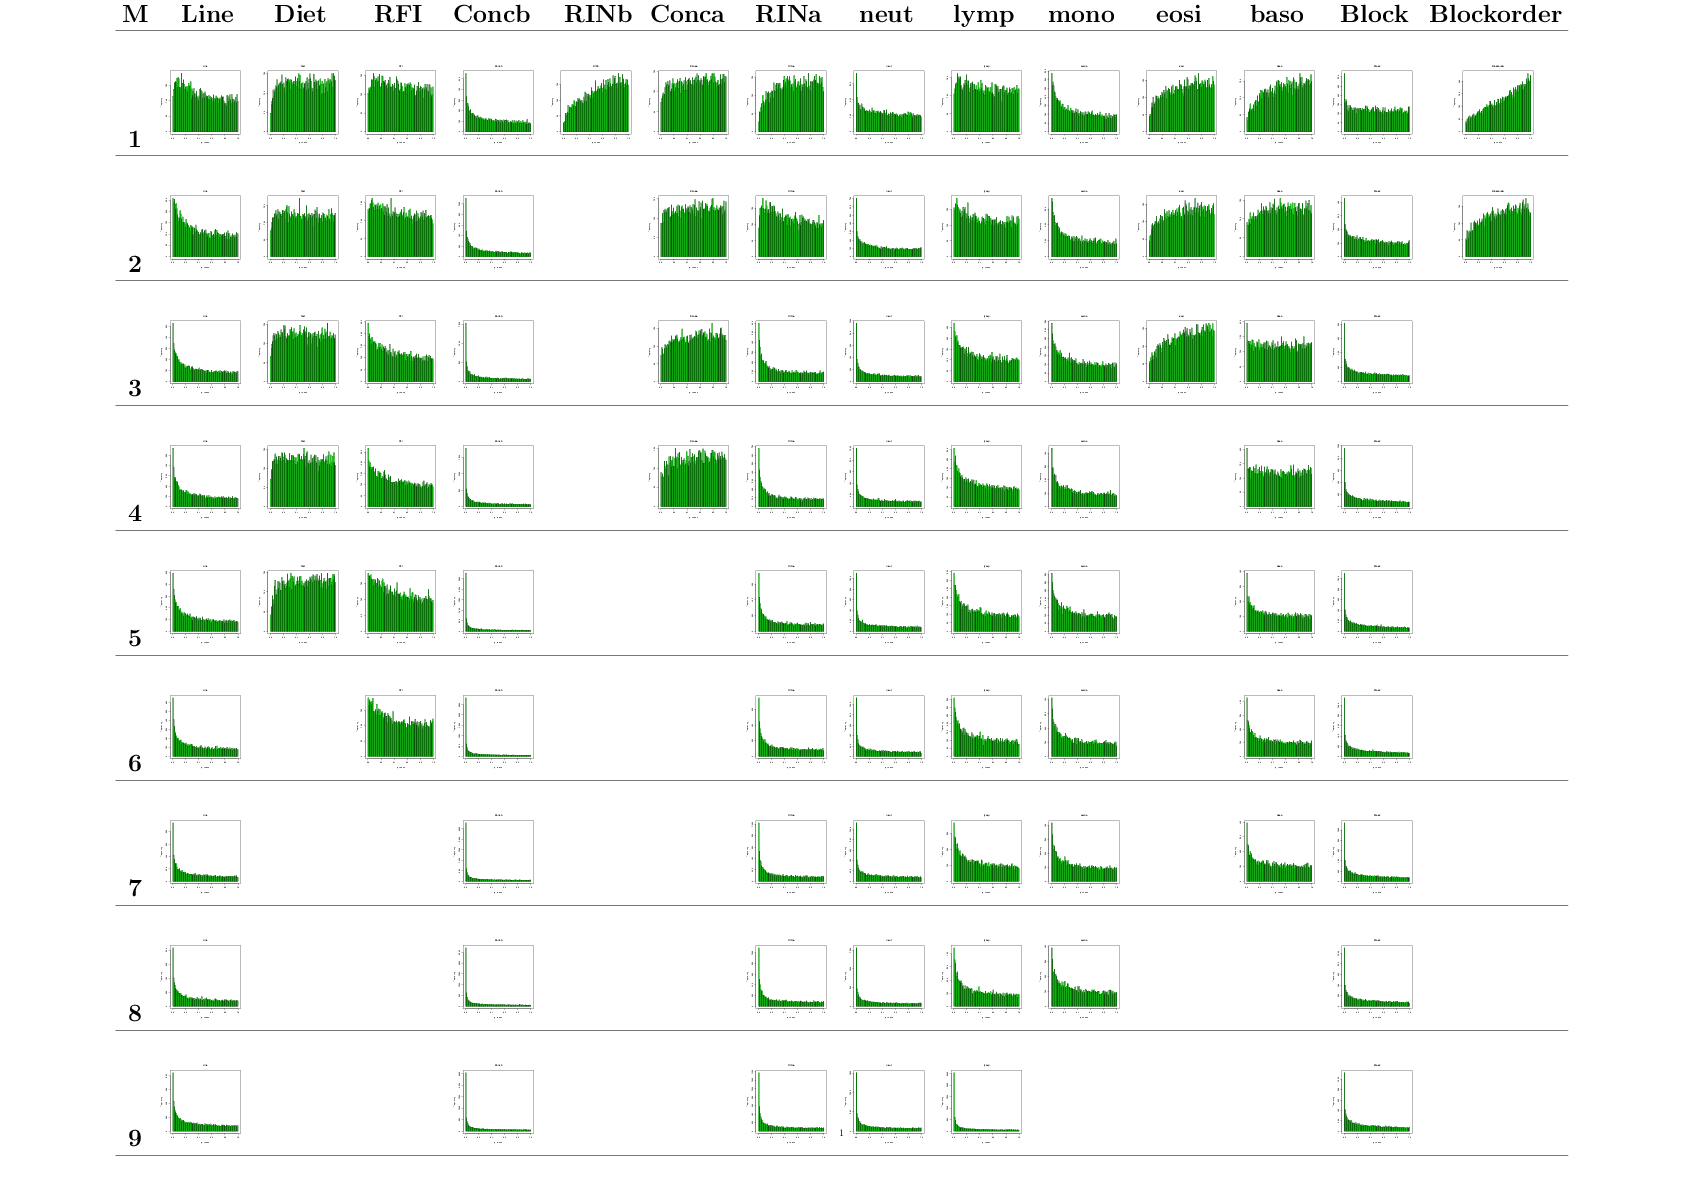
\includegraphics[scale = 0.22]{PlotG9P2PairedEndCBCpvalue05.png}
\caption{The plot shows models obtained from the backward model selection procedure $pvalue05$ when applying the procedure to  the RNA-Seq from RFI project.}
\label{pvalue05}
\end{figure}


\begin{figure}[H]
\centering
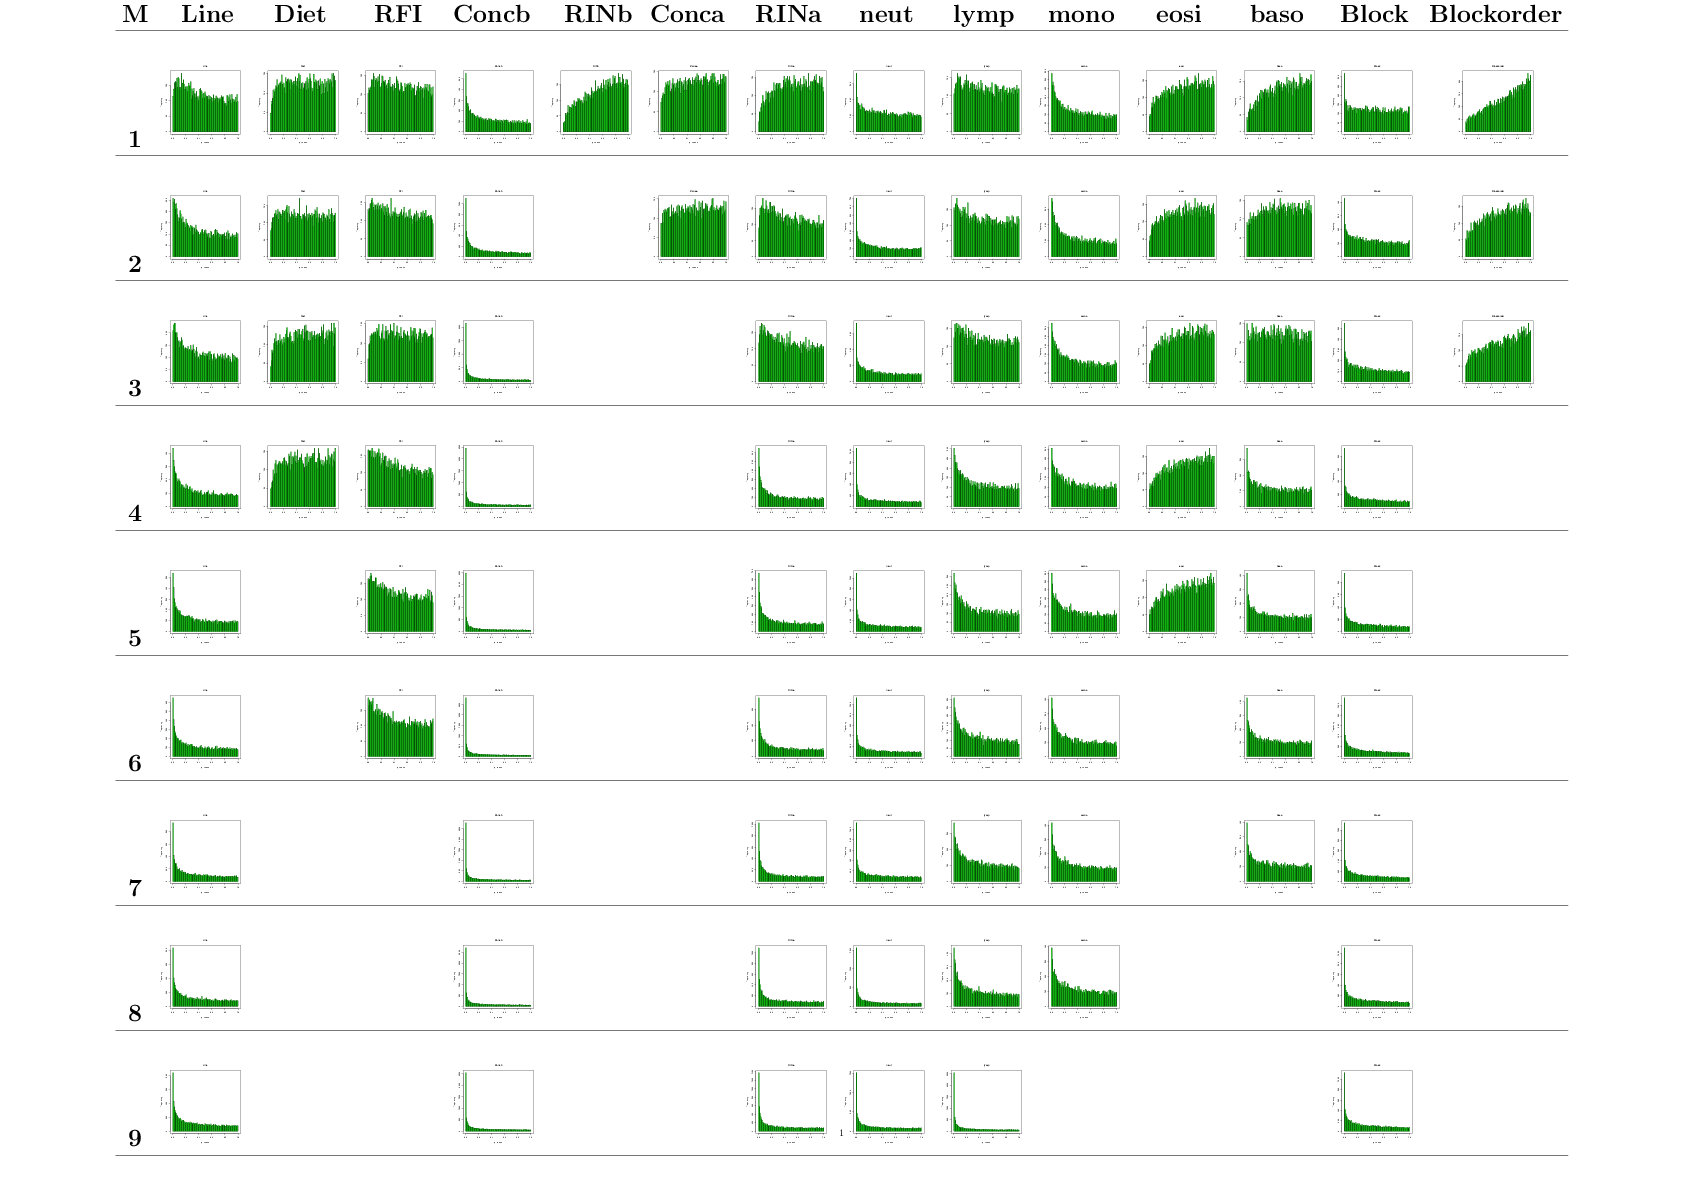
\includegraphics[scale = 0.22]{PlotG9P2PairedEndCBCks.png}
\caption{The plot shows models obtained from the backward model selection procedure $ks$ when applying the procedure to the RNA-Seq from RFI project. }
\label{ks}
\end{figure}


\section{ Simulation Justification based on Real Data}
Due to the complexity of the experiment design which involves many nuisance covariates, we are going to perform only simulation study based on the real data. By doing this, the simulation data will have structure similar to the real data. Specifically, we collect estimates coefficients of the intercepts, the main effect Line, and the other nuisance covariates in the log(mean) formula of the optimal model which is model M7 chosen from the backward selection procedures. Also, we collect  the estimate of  number of true null $m_{0}$ for Line effect,  the estimates of the negative binomial dispersion parameters, and the $q$-values of all genes for all tests of main effect and the nuisance covariates.

The simulation is proceeded as below. Suppose the fitted of log(mean)  from the optimal  Model 7 is 

\begin{align}\label{eq1}
\log(\mu_{gij}) = & o_{ij} +\hat{\alpha}_g + \hat{\beta}_{g,Line}*I(Line) \notag\\
     & +  \hat{\beta}_{g,Concb}*Concb +  \hat{\beta}_{g,RINa}*RINa + \hat{\beta}_{g,neut}*neut \notag \\
     & + \hat{\beta}_{g,lymp}*lymp + \hat{\beta}_{g,mono}*mono + \hat{\beta}_{g,baso}*baso \notag\\
    &  + \hat{\beta}_{g,Block}*I(Block).
\end{align}

We set the coefficient $\hat{\beta}_{g,Line} = 0$ for each gene $g$ in the set of $m_{0Line}$ genes which are genes having largest  $q$ values of Line effect. We denote the gene indexes corresponding to the new non-zero $\hat{\beta}_{g,Line}$ as $DEgenelist$ which is a subset of $Genelist :=\{1, 2, \dots, 12280\}$. Set $EEgenelist = Genelist\setminus DEgenelist$. The other coefficients are unchanged. Using those new coefficients, the new mean $\hat{\mu}_{gij}$  of count data  is calculated according to the formula \eqref{eq1} for each gene and each sample. Suppose that the estimates of negative binomial dispersion parameters for all genes in Model 7 are $\hat{\omega}_{g}, g = 1, \dots, m$ . We simulate 100 data sets, each of those consists of 5000 genes with different  $\pi$  which is the proportion of equivalently expressed  genes between lines. We consider 4 scenarios of $\pi$ which are $ \pi = 0.9, 0.8, 0.7, 0.6$. The simulation steps  are described as below. 
\begin{itemize}
\item[1. ] Denote the number of equivalently expressed genes and the number of differently expressed genes between two Lines as $EE, DE$, respectively, and $EE = 5000\pi$, $DE = 5000-EE$.

\item[2. ] Randomly sample $EE$ indexes $g^{(0)}_1, \dots, g^{(0)}_{EE}$ from the set $EEgenelist$, and $DE$ indexes $g^{(1)}_1, \dots, g^{(1)}_{DE}$ from the set $DEgenelist$.

\item[3.] For each $g \in \{ g^{(0)}_1, \dots, g^{(0)}_{EE}, g^{(1)}_1, \dots, g^{(1)}_{DE}\}$, and $i = 1, 2$, $j = 1, \dots, n_i $,  simulate the count data $y_{gij}$ from $\mbox{NegBin}(\hat{\mu}_{gij}, \hat{\omega}_{g})$ for gene $g$ in treatment group $i$ and replication $j$. The simulated counts are arranged in the form of 5000$\times 31$ table, where the fist $EE$ rows are equivalently expressed genes, the last $DE$ rows are differentially expressed genes.

\item[4. ] Apply the backward selection procedures $pvalue05$ and $ks$ to the simulated count data set with Line effect and all nuisance covariates (Diet, RFI, Concb, RINb, Conca, RINa, lymp, neut, mono, baso, eosi, Block, Order) to get the optimal model for  differential expression analysis  between two lines. A gene is declared to be differentially expressed if its $q$-value is less than or equal 0.05.

\item[5. ] Compute the False Discovery Proportion (FDP), number of true discovery (S), and the partial area under the receiver operating  characteristic curve (PAUC) corresponding to the false positive rate less than or equal 0.05. 

\item[6.] Calculate average of  S, PAUC, and calculate FDR which is the average of FDP over 100 simulation and the standard errors of those quantities.

\item[7. ] Do the same things as steps 4, 5, 6 for the other traditional approaches: fitting only Line effect (L), fitting Line effect and all nuisance covariates (F), fitting the oracle method (O)  which is the model generating the simulated data. 
\end{itemize}

The simulation results based on 100 data sets are summarized in Figure \ref{simfigure},  and Table \ref{simpvalue05} and Table \ref{simks}. Figure \ref{simfigure} shows that the proposed backward selection procedure methods (either $pvalue05$ or $ks$)  control FDR well. The proposed methods also have higher power  by means of  measurement of partial area under the ROC curve PAUC or number of true rejections S) in comparison to the traditional approach  which  ignores (L) or includes all  (F) nuisance covariates. The performance of our backward selection procedure methods is very similar to that of oracle method. Table \ref{simpvalue05} and Table \ref{simks} show that either $pvalue05$ or $ks$ backward selection procedure method can detect the true underlying model of data generating process with very high probability. 

\begin{figure}
\centering
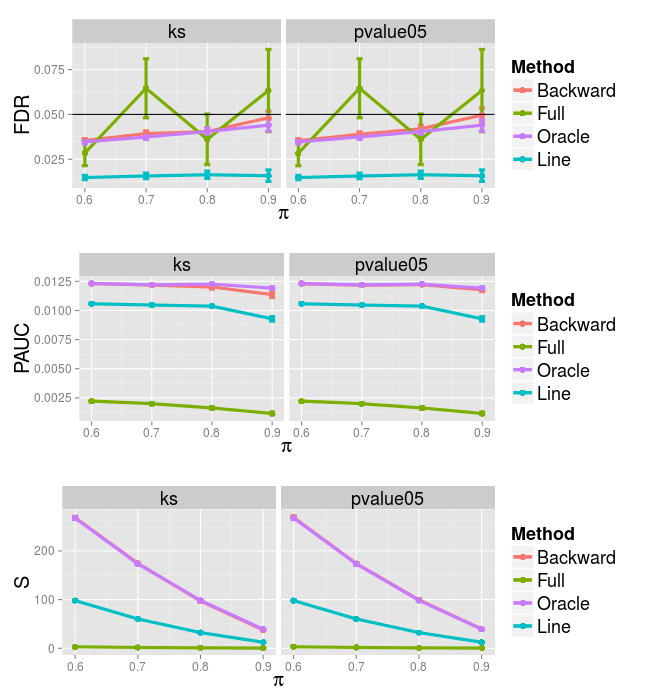
\includegraphics[scale = 0.8]{result.png}
\caption{The true false discovery rate FDR, the partial area under the receiver operating characteristics curve PAUC, and the number of true rejections S, as well as their standard error based on  100 simulation data sets are calculated for  $\pi = 0.9, 0.8, 0.7, 0.6$. B, F, O, L, stand for Backward selection procedure method which includes Line effect and important nuisance covariate based on backward selection procedures, Full model method which includes all covairates, Oracle model method which includes the true covariates, and Line model method which includes only Line effect.}
\label{simfigure}
\end{figure}

\begin{table}
\centering
{\scriptsize
\begin{tabular}{|c|c|c|c|c|c|c|c|c|c|c|c|c|c|c|c|}
  \hline
$\pi$ & Line & Diet & RFI & Concb & RINb & Conca & RINa & neut & lymp & mono & eosi & baso & Block & Order & pvalue05 \\ 
  \hline
0.9 & 1 & 0 & 0 & 1 & 0 & 1 & 1 & 1 & 1 & 1 & 0 & 1 & 1 & 0 & 3 \\ 
  0.9 & 1 & 0 & 0 & 1 & 0 & 1 & 1 & 1 & 1 & 1 & 1 & 1 & 1 & 0 & 1 \\ 
  0.9 & 1 & 0 & 0 & 1 & 0 & 0 & 1 & 1 & 1 & 1 & 0 & 1 & 1 & 0 & 74 \\ 
  0.9 & 1 & 0 & 0 & 1 & 0 & 0 & 1 & 1 & 1 & 1 & 1 & 1 & 1 & 0 & 9 \\ 
  0.9 & 1 & 0 & 0 & 1 & 1 & 1 & 1 & 1 & 1 & 1 & 0 & 1 & 1 & 0 & 1 \\ 
  0.9 & 1 & 0 & 0 & 1 & 1 & 0 & 1 & 1 & 1 & 1 & 0 & 1 & 1 & 0 & 4 \\ 
  0.9 & 1 & 0 & 0 & 1 & 1 & 0 & 1 & 1 & 1 & 1 & 1 & 1 & 1 & 0 & 1 \\ 
  0.9 & 1 & 1 & 0 & 1 & 0 & 1 & 1 & 1 & 1 & 1 & 1 & 1 & 1 & 0 & 1 \\ 
  0.9 & 1 & 1 & 0 & 1 & 0 & 0 & 1 & 1 & 1 & 1 & 1 & 1 & 1 & 0 & 4 \\ 
  0.9 & 1 & 1 & 0 & 1 & 1 & 1 & 1 & 1 & 1 & 1 & 1 & 1 & 1 & 0 & 1 \\ 
  0.9 & 1 & 1 & 1 & 1 & 0 & 0 & 1 & 1 & 1 & 1 & 0 & 1 & 1 & 0 & 1 \\ 
   \hline
0.8 & 1 & 0 & 0 & 1 & 0 & 1 & 1 & 1 & 1 & 1 & 0 & 1 & 1 & 0 & 2 \\ 
  0.8 & 1 & 0 & 0 & 1 & 0 & 0 & 1 & 1 & 1 & 1 & 0 & 1 & 1 & 0 & 74 \\ 
  0.8 & 1 & 0 & 0 & 1 & 0 & 0 & 1 & 1 & 1 & 1 & 1 & 1 & 1 & 0 & 5 \\ 
  0.8 & 1 & 0 & 0 & 1 & 1 & 1 & 1 & 1 & 1 & 1 & 0 & 1 & 1 & 0 & 2 \\ 
  0.8 & 1 & 0 & 0 & 1 & 1 & 0 & 1 & 1 & 1 & 1 & 0 & 1 & 1 & 0 & 5 \\ 
  0.8 & 1 & 0 & 0 & 1 & 1 & 0 & 1 & 1 & 1 & 1 & 1 & 1 & 1 & 0 & 1 \\ 
  0.8 & 1 & 1 & 0 & 1 & 0 & 1 & 1 & 1 & 1 & 1 & 0 & 1 & 1 & 0 & 1 \\ 
  0.8 & 1 & 1 & 0 & 1 & 0 & 0 & 1 & 1 & 1 & 1 & 0 & 1 & 1 & 0 & 7 \\ 
  0.8 & 1 & 1 & 0 & 1 & 0 & 0 & 1 & 1 & 1 & 1 & 1 & 1 & 1 & 0 & 3 \\ 
   \hline
0.7 & 1 & 0 & 0 & 1 & 0 & 1 & 1 & 1 & 1 & 1 & 0 & 1 & 1 & 0 & 2 \\ 
  0.7 & 1 & 0 & 0 & 1 & 0 & 0 & 1 & 1 & 1 & 1 & 0 & 1 & 1 & 0 & 78 \\ 
  0.7 & 1 & 0 & 0 & 1 & 0 & 0 & 1 & 1 & 1 & 1 & 1 & 1 & 1 & 0 & 10 \\ 
  0.7 & 1 & 0 & 0 & 1 & 1 & 0 & 1 & 1 & 1 & 1 & 0 & 1 & 1 & 0 & 3 \\ 
  0.7 & 1 & 0 & 0 & 1 & 1 & 0 & 1 & 1 & 1 & 1 & 1 & 1 & 1 & 0 & 1 \\ 
  0.7 & 1 & 1 & 0 & 1 & 0 & 0 & 1 & 1 & 1 & 1 & 0 & 1 & 1 & 0 & 5 \\ 
  0.7 & 1 & 1 & 0 & 1 & 1 & 0 & 1 & 1 & 1 & 1 & 1 & 1 & 1 & 0 & 1 \\ 
   \hline
0.6 & 1 & 0 & 0 & 1 & 0 & 1 & 1 & 1 & 1 & 1 & 0 & 1 & 1 & 0 & 2 \\ 
  0.6 & 1 & 0 & 0 & 1 & 0 & 0 & 1 & 1 & 1 & 0 & 0 & 1 & 1 & 0 & 1 \\ 
  0.6 & 1 & 0 & 0 & 1 & 0 & 0 & 1 & 1 & 1 & 1 & 0 & 1 & 1 & 0 & 78 \\ 
  0.6 & 1 & 0 & 0 & 1 & 0 & 0 & 1 & 1 & 1 & 1 & 1 & 1 & 1 & 0 & 9 \\ 
  0.6 & 1 & 0 & 0 & 1 & 1 & 0 & 1 & 1 & 1 & 1 & 1 & 1 & 1 & 0 & 1 \\ 
  0.6 & 1 & 1 & 0 & 1 & 0 & 0 & 1 & 1 & 1 & 1 & 0 & 1 & 1 & 0 & 6 \\ 
  0.6 & 1 & 1 & 0 & 1 & 0 & 0 & 1 & 1 & 1 & 1 & 1 & 1 & 1 & 0 & 1 \\ 
  0.6 & 1 & 1 & 0 & 1 & 1 & 1 & 1 & 1 & 1 & 1 & 0 & 1 & 1 & 0 & 1 \\ 
  0.6 & 1 & 1 & 0 & 1 & 1 & 1 & 1 & 1 & 1 & 1 & 1 & 1 & 1 & 0 & 1 \\ 
   \hline
\end{tabular}
}
\caption{Summary of Final Model selected by Backward Selection procedure $pvalue05$.} 
\label{simpvalue05}
\end{table}


\begin{table}
\centering
{\scriptsize
\begin{tabular}{|c|c|c|c|c|c|c|c|c|c|c|c|c|c|c|c|}
  \hline
$\pi$ & Line & Diet & RFI & Concb & RINb & Conca & RINa & neut & lymp & mono & eosi & baso & Block & Order & ks \\ 
  \hline
0.9 & 1 & 0 & 0 & 1 & 0 & 1 & 1 & 1 & 1 & 1 & 1 & 1 & 1 & 0 & 1 \\ 
  0.9 & 1 & 0 & 0 & 1 & 0 & 0 & 1 & 1 & 1 & 1 & 0 & 1 & 1 & 0 & 69 \\ 
  0.9 & 1 & 0 & 0 & 1 & 0 & 0 & 1 & 1 & 1 & 1 & 0 & 1 & 1 & 1 & 4 \\ 
  0.9 & 1 & 0 & 0 & 1 & 0 & 0 & 1 & 1 & 1 & 1 & 1 & 1 & 1 & 0 & 9 \\ 
  0.9 & 1 & 0 & 0 & 1 & 1 & 0 & 1 & 1 & 1 & 1 & 0 & 1 & 1 & 0 & 6 \\ 
  0.9 & 1 & 1 & 0 & 1 & 0 & 1 & 1 & 1 & 1 & 1 & 1 & 1 & 1 & 0 & 2 \\ 
  0.9 & 1 & 1 & 0 & 1 & 0 & 0 & 1 & 1 & 1 & 1 & 0 & 1 & 1 & 0 & 1 \\ 
  0.9 & 1 & 1 & 0 & 1 & 0 & 0 & 1 & 1 & 1 & 1 & 1 & 1 & 1 & 0 & 2 \\ 
  0.9 & 1 & 1 & 0 & 1 & 1 & 1 & 1 & 1 & 1 & 1 & 1 & 1 & 1 & 0 & 1 \\ 
  0.9 & 1 & 1 & 0 & 1 & 1 & 0 & 1 & 1 & 1 & 1 & 0 & 1 & 1 & 0 & 1 \\ 
  0.9 & 1 & 1 & 1 & 1 & 1 & 1 & 1 & 1 & 1 & 1 & 0 & 1 & 1 & 0 & 1 \\ 
  0.9 & 1 & 1 & 1 & 1 & 1 & 1 & 1 & 1 & 1 & 1 & 1 & 1 & 1 & 1 & 3 \\ 
   \hline
0.8 & 1 & 0 & 0 & 1 & 0 & 1 & 1 & 1 & 1 & 1 & 0 & 1 & 1 & 0 & 2 \\ 
  0.8 & 1 & 0 & 0 & 1 & 0 & 1 & 1 & 1 & 1 & 1 & 1 & 1 & 1 & 0 & 1 \\ 
  0.8 & 1 & 0 & 0 & 1 & 0 & 0 & 1 & 1 & 1 & 1 & 0 & 1 & 1 & 0 & 77 \\ 
  0.8 & 1 & 0 & 0 & 1 & 0 & 0 & 1 & 1 & 1 & 1 & 1 & 1 & 1 & 0 & 7 \\ 
  0.8 & 1 & 0 & 0 & 1 & 1 & 0 & 1 & 1 & 1 & 1 & 0 & 1 & 1 & 0 & 2 \\ 
  0.8 & 1 & 0 & 0 & 1 & 1 & 0 & 1 & 1 & 1 & 1 & 1 & 1 & 1 & 0 & 1 \\ 
  0.8 & 1 & 1 & 0 & 1 & 0 & 0 & 1 & 1 & 1 & 1 & 0 & 1 & 1 & 0 & 7 \\ 
  0.8 & 1 & 1 & 0 & 1 & 0 & 0 & 1 & 1 & 1 & 1 & 1 & 1 & 1 & 0 & 1 \\ 
  0.8 & 1 & 1 & 1 & 1 & 1 & 1 & 1 & 1 & 1 & 1 & 1 & 1 & 1 & 1 & 2 \\ 
   \hline
0.7 & 1 & 0 & 0 & 1 & 0 & 1 & 1 & 1 & 1 & 1 & 0 & 1 & 1 & 0 & 2 \\ 
  0.7 & 1 & 0 & 0 & 1 & 0 & 0 & 1 & 1 & 1 & 1 & 0 & 1 & 1 & 0 & 79 \\ 
  0.7 & 1 & 0 & 0 & 1 & 0 & 0 & 1 & 1 & 1 & 1 & 1 & 1 & 1 & 0 & 8 \\ 
  0.7 & 1 & 0 & 0 & 1 & 1 & 0 & 1 & 1 & 1 & 1 & 0 & 1 & 1 & 0 & 2 \\ 
  0.7 & 1 & 0 & 0 & 1 & 1 & 0 & 1 & 1 & 1 & 1 & 1 & 1 & 1 & 0 & 2 \\ 
  0.7 & 1 & 1 & 0 & 1 & 0 & 0 & 1 & 1 & 1 & 1 & 0 & 1 & 1 & 0 & 4 \\ 
  0.7 & 1 & 1 & 0 & 1 & 0 & 0 & 1 & 1 & 1 & 1 & 1 & 1 & 1 & 0 & 2 \\ 
  0.7 & 1 & 1 & 0 & 1 & 1 & 0 & 1 & 1 & 1 & 1 & 1 & 1 & 1 & 0 & 1 \\ 
   \hline
0.6 & 1 & 0 & 0 & 1 & 0 & 1 & 1 & 1 & 1 & 1 & 0 & 1 & 1 & 0 & 1 \\ 
  0.6 & 1 & 0 & 0 & 1 & 0 & 0 & 1 & 1 & 1 & 1 & 0 & 1 & 1 & 0 & 82 \\ 
  0.6 & 1 & 0 & 0 & 1 & 0 & 0 & 1 & 1 & 1 & 1 & 1 & 1 & 1 & 0 & 8 \\ 
  0.6 & 1 & 0 & 0 & 1 & 1 & 0 & 1 & 1 & 1 & 1 & 0 & 1 & 1 & 0 & 1 \\ 
  0.6 & 1 & 1 & 0 & 1 & 0 & 0 & 1 & 1 & 1 & 1 & 0 & 1 & 1 & 0 & 4 \\ 
  0.6 & 1 & 1 & 0 & 1 & 0 & 0 & 1 & 1 & 1 & 1 & 1 & 1 & 1 & 0 & 3 \\ 
  0.6 & 1 & 1 & 0 & 1 & 1 & 1 & 1 & 1 & 1 & 1 & 0 & 1 & 1 & 0 & 1 \\ 
   \hline
\end{tabular}
}
\caption{Summary of Final Model selected by Backward Selection procedure $ks$.} 
\label{simks}
\end{table}
\newpage
\section{ Conclusion}
The backward selection procedures discussed in this paper provide a simple and comparatively effective method in differential expression analysis accounting for many nuisance covariates. In our simulation study, the proposed methods outperform the traditional approaches such as method including or excluding all nuisance covariate. 


\section*{ Acknowledgments}
This material is based upon work supported by Agriculture and Food
Research Initiative Competitive Grant No. 2011-68004-30336 from
the USDA National Institute of Food and Agriculture, and the
National Science Foundation (NSF) under Grant No. 0922746.
Any opinions, findings, and conclusions or recommendations expressed in this material are those of the authors and do not necessarily reflect the views of the USDA or NSF.

Yet Nguyen was funded in part by a grant from the Vietnam Education Foundation (VEF). The opinions, findings, and conclusions stated herein are those of the authors and do not necessarily reflect those of VEF.


\bibliographystyle{ECA_jasa}
\bibliography{bibjabes}

\end{document}
